\scanpage{8}
Supposons que $q\alpha-\alpha'\ne0$ alors
\[
\begin{aligned}
(1)\ \Longrightarrow\quad &p\mid\sum_{i=1}^{q-1}C_q^i\,a^i b'^{\,q-i-1}+b'^{\,q-1}\\
\Longrightarrow\quad &p\mid q\,a^{q-1}\qquad\text{car }p\mid b'\ \text{et pour }i\ne q-1\quad q-i-1\deleted{\ne0}>0
\end{aligned}
\]
or $p\mid b'$ et $b'\mid b^q$ donc $b'\mathrel{\underset{1}{\smile}}a$ donc $p\mathrel{\underset{1}{\smile}}a$

\deleted{donc si $\unsure{p\ne1|p\ne q}$}
\[
(1)\ \Longrightarrow\quad p\mid q\qquad\text{donc }\deleted{p=1\ \text{ou }}p=q\quad(\text{si }q\alpha-\alpha'\ne0)
\]
Donc si $p\ne q$ \quad $p$ premier \inserted{ou $p=1$} et $p\mid b'$ alors $\alpha'=q\alpha$
% The parenthetical cancellation has two distinct oblique strokes.
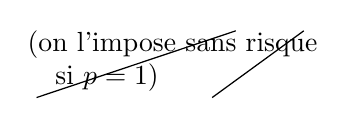
\begin{tikzpicture}[baseline=(n.north)]
\node[inner sep=0pt,align=left] (n) {\rlap{\begin{tabular}{@{}l@{}}(on l'impose sans risque\\\quad si $p=1$)\end{tabular}}\phantom{\begin{tabular}{@{}l@{}}\deleted{(on l'impose sans risque}\\\quad\deleted{si $p=1$)}\end{tabular}}};
\draw[line width=.45pt] ([xshift=.12cm,yshift=-.03cm]n.south west) -- ([xshift=2.65cm,yshift=-.04cm]n.north west);
\draw[line width=.45pt] ([xshift=2.35cm,yshift=-.03cm]n.south west) -- ([xshift=-.18cm,yshift=-.04cm]n.north east);
\end{tikzpicture}

Donc $\exists\,b_0\in\mathbb N^*$ et $\exists\,\gamma\in\mathbb N$ tel que $b'=q^\gamma b_0^q$ \margin{$q\nmid b_0$}

de plus $b_0\mid b$ et si $b=b_0 b''$ alors $b_0\mathrel{\underset{1}{\smile}}b''$ ?

De même $\exists\,a_0\in\mathbb N^*$ et $\exists\,\unsure{\zeta|\delta}\in\mathbb N$ tel que $a'=q^\zeta a_0^q$ avec $a_0\mid a$ et si $a=a_0a''$ alors $a_0\mathrel{\underset{1}{\smile}}a''$ ?

or $a\mathrel{\underset{1}{\smile}}b\Longrightarrow a_{\deleted{\unsure{0}}}'\mathrel{\underset{1}{\smile}}b'\Longrightarrow\zeta\times\gamma=0$ (et aussi $a_0\mathrel{\underset{1}{\smile}}b_0$)

Je suppose désormais que $\zeta=0$ donc $a'=a_0^q$

Donc \quad $c=b+a_0^q=a+q^\gamma b_0^q$
\margin{\begin{tikzpicture}[baseline=(n.base)]
\node[inner sep=2pt,text width=.85\marginparwidth] (n) {pour $q=2$ on a, $a_0=b_0=1$, $\gamma=1$, $b=4$, $a=3$, $c=5$};
\draw (n.north east) -- (n.north west) -- (n.south west) -- (n.south east);
\end{tikzpicture}}

\noindent\rule{\linewidth}{.35pt}\par
Je fais l'hypothése suivante \quad si $q$ premier et $1\leqslant i<q$ alors $q\mid C_q^i$
\par\noindent\rule{\linewidth}{.35pt}\par
alors Si $q\geqslant3$ et $q\alpha-\alpha'\geqslant2$ \deleted{\unsure{alors}} on a
% Two separate curved marks follow the pale p=q. The lower one's role is unresolved.
\inserted{$p=q\,\underset{\hspace{.2em}\unsure{,}}{,}\ {\unsure{a|\alpha}}'=\gamma$}
\[
\begin{aligned}
(1)\ \Longrightarrow\quad &\deleted{\unsure{p^{2}|p}}q^2\mid q\,a^{q-1}\quad
\text{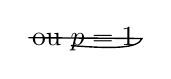
\begin{tikzpicture}[baseline=(n.base)]
\node[inner sep=0pt] (n) {\rlap{ou $p=1$}\phantom{\deleted{ou $p=1$}}};
\draw[line width=.5pt] ([xshift=-.04cm,yshift=.02cm]n.west) -- ([xshift=.08cm,yshift=.01cm]n.east) .. controls ([xshift=.03cm,yshift=-.12cm]n.east) and ([xshift=-.3cm,yshift=-.12cm]n.east) .. ([xshift=.50cm,yshift=-.08cm]n.west);
\end{tikzpicture}}
\quad
% Faint residual strokes and points in the interline gap; no character is supplied.
\begin{tikzpicture}[baseline=-.05cm,x=1cm,y=1cm]
\draw[gray,line width=.35pt] (0,.12) .. controls (.10,.02) and (.18,-.02) .. (.31,.02);
\draw[gray,line width=.35pt] (.21,.13) -- (.27,.10);
\draw[gray,line width=.35pt] (.34,.02) .. controls (.40,.17) and (.42,.26) .. (.52,.24);
\draw[gray,line width=.35pt] (.49,.15) -- (.64,.14);
\fill[gray] (.58,.31) circle (.5pt);
\fill[gray] (.64,.04) circle (.45pt);
\fill[gray] (.69,-.02) circle (.45pt);
\end{tikzpicture}
\\
\Longrightarrow\quad&q\mid a^{q-1}\quad
\overset{\inserted{\text{absurde car }q\nmid a}}{\text{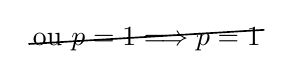
\begin{tikzpicture}[baseline=(n.base)]
\node[inner sep=0pt] (n) {\rlap{ou $p=1\Longrightarrow p=1$}\phantom{\deleted{ou $p=1\Longrightarrow p=1$}}};
\draw[line width=.6pt] ([xshift=-.05cm,yshift=-.06cm]n.west) -- ([xshift=.04cm,yshift=.12cm]n.east);
\end{tikzpicture}}}
\end{aligned}
\]
Donc $\gamma=0$ ou $\gamma=
% Cancelled q, raised q alpha minus one, and repeated oblique return strokes.
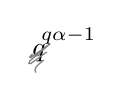
\begin{tikzpicture}[baseline=(q.base),x=1ex,y=1ex]
\node[inner sep=0pt] (q) at (0,0) {\rlap{$q$}\phantom{\deleted{$q$}}};
\node[inner sep=0pt,anchor=south west] at (.15,.75) {$\scriptstyle q\alpha-1$};
\draw[gray,line width=.45pt] (-.55,-.05) .. controls (-.77,-.29) and (-.90,-.39) .. (-.70,-.35) -- (.95,.82) -- (-.77,-.63) .. controls (-.90,-.81) and (-.87,-.90) .. (-.70,-.86) -- (.65,.12);
\draw[gray,line width=.45pt] (.40,-.56) .. controls (-.10,-.95) and (-.35,-1.16) .. (-.34,-1.43) .. controls (-.35,-1.53) and (-.31,-1.57) .. (-.25,-1.60);
\end{tikzpicture}$ (sous réserve que l'hypothése est vraie)%
\margin{\begin{tikzpicture}[baseline=(n.base)]
\node[inner sep=0pt,text width=.85\marginparwidth] (n) {C'est peut-être interessant car ici $2$ est mis à part dans l'ensemble des nombres premiers};
% A small detached point is visible at the lower start of the return arrow.
\fill (n.south east) circle (.45pt);
\draw[->] ([xshift=.07cm]n.south east) -- ([xshift=.16cm]n.south east) |- (n.north east);
\end{tikzpicture}}
% archive sheet number: 7
